%------------------------------------------------
\section{Contributions}
%------------------------------------------------

% Intro à refaire 
%-----------------------------------------------------------------
\subsection{Relations aux triangulations de Delaunay}
%-----------------------------------------------------------------


L'enveloppe convexe est unique. Les algorithmes implantés fournissent les sommets dans l'ordre trigonométrique. Il est possible de reconstruire le polygone convexe et d'en déduire ses arêtes. Elles se décomposent en motif de droites discrètes. Un motif de droite discrète est inclue dans les segments de droites discrètes. La triangulation de Delaunay de ces motifs est connue. \cite{RoussillonL11}\\

\begin{figure}[H]
  \centering
  \includegraphics[width=0.5\linewidth]{fig/5-con/tri/con-motif-0.pdf}
  \caption{Triangulation de Delaunay d'un motif de droite discrète}
\end{figure}

La triangulation de Delaunay dépend des convergents. Le dernier convergent n'appartenant pas au segment de droite discrète est le sommet du triangle incident de la triangulation de Delaunay. Il est appelé le point de bézout. À l'aide d'un calcul récursif, il est possible de construire l'intégralité de la triangulation de Delaunay.

\begin{figure}[H]
  \centering
  \includegraphics[width=0.5\linewidth]{fig/5-con/tri/con-conv-0.pdf}
  \caption{Calcul de convergents et triangulations de Delaunauy}
\end{figure}

Comme les convergents sont calculés dans l’algorithme de Har-Peled, il est probable de pouvoir construire l'$\alpha$-shape directement. 

%-----------------------------------------------------------------
\subsection{$\alpha$-shape, $\alpha \leq 0$ - Généralisation de Har-Peled}
%-----------------------------------------------------------------

%-----------------------------------------------------------------
\subsubsection{Construction de l'algorithme}

La méthode de calcul de l'$\alpha$-shape pour $\alpha <0$ reproduit le schéma du calcul de l’enveloppe convexe. Il y a cependant une étape supplémentaire pour chaque convergent à l'intérieur du disque afin de contrôler la possibilité d'avoir construit une arête de l'$\alpha$-shape.

L'algorithme commence similairement à l'enveloppe convexe avec la recherche d'un point de départ. La même méthode est utilisée pour trouver le point $a$ d'ordonnée minimale et d'abscisse maximale. Comme il appartient à l'enveloppe convexe, il appartient également à l'$\alpha$-shape.

À partir de ce point, nous lançons une série de convergents pour récupérer les sommets $e$ potentiels. Les convergents se trouvent alternativement à l'intérieur de disque (convergent de degré impaire) et à l'extérieur où exactement sur le bord du disque (convergent de degré pair). À chaque convergent à l'intérieur (de couleur bleue foncé), on contrôle la possibilité d'avoir trouvé un sommet.

Soient  $b = p_{k-2} + (q_k - 1) * p_{k-1}$ et $c = p_k = p_{k-2} + q_k * p_{k-1}$. Pour savoir si c est un sommet, nous utilisons un prédicat qui compare la taille du rayon \textbf{$R_T$} du cercle circonscrit au triangle : $T(a, b, c)$ à la taille du rayon de notre disque généralisé : \textbf{$R_{\alpha}$} $= -1/\alpha$. Il faut distinguer deux cas de figures.\\

\begin{figure}[H]
  \centering
  \includegraphics[width=0.45\linewidth]{fig/5-con/nas/con-nas-0.pdf}
  \includegraphics[width=0.45\linewidth]{fig/5-con/nas/con-nas-1.pdf}
  \caption{Calcul des convergents et du Prédicat}
\end{figure}

Si $\alpha = \alpha_{2}$ (en jaune) alors \textbf{$R_{\alpha_{2}} < R_T$} et le point b appartient au notre disque généralisé de rayon $-1/R_{\alpha_{2}}$ ( b appartient au complémentaire du disque de rayon $1/R_{\alpha_{2}}$). On ne sait pas encore si le convergent c sera un sommet de l'$\alpha$-shape, mais on sait que b n'en sera pas un. Nous pouvons continuer le calcul des convergents.\\ 

Si $\alpha = \alpha_{1}$ (en violet) alors \textbf{$R_{\alpha_{1}} > R_T$} et le point b n'appartient pas à notre disque généralisé de rayon $-1/R_{\alpha_{1}}$. L'$\alpha$-hull ne peut rejoindre c par a sans au moins passé par b. b et c appartiennent à notre $\alpha$-shape. Il faut maintenant vérifier si les points $b_i = p_{k-2} + i*p_{k-1} \forall i \in [0, q_k-2]$ appartiennent également à l'$\alpha$-shape. \\

De part la construction des triangles, la taille des rayons de leur cercle circonscrit $R_{T_{i}}$ est croissante. Il suffit de tester le dernier avec le plus grand cercle pour savoir si nous pouvons continuer notre algorithme et lancer les convergents suivants ou si nous devons déterminer quel sera le point $\alpha$-extrême par une recherche dichotomique. La recherche dichotomique permet de trouver en $log(q_k)$ le triangle adéquate $T_i = (a, b_{i}, b_{i+1}$ tel que $R_{T_i} > R_{\alpha}$ et $R_{T_{i-1}} \leq R_{\alpha}$.

\begin{figure}[H]
  \centering
  \includegraphics[trim = 1.2cm 1.2cm 1.2cm 0.6cm, clip,width=\linewidth]{fig/5-con/nas/con-nas-dicho.pdf}
  \caption{Taille croissante des rayons des cerlces circonscrits au triangle.}
\end{figure}

Le triangle renvoyé par la méthode dichotomique assure que l'ensemble des points $\left\{ b_{i},\ldots, b_{q_k}, c \right\}$ appartiennent à l'$\alpha$-shape. Nous continuons la méthode en repartant du sommet c.
 
\begin{figure}[H]
  \centering
  \includegraphics[trim = 1.2cm 1.2cm 1.2cm 0.6cm, clip,width=\linewidth]{fig/5-con/nas/con-nas-2.pdf}
  \caption{Nouveaux points et sommets de l'$\alpha$-shape.}
\end{figure}


%-----------------------------------------------------------------
\subsubsection{Résultats}

Les processus de création des disques $\mathcal{D}$ est le même que lors du calcul de l'enveloppe convexe. Néanmoins, pour chaque disque il est possible de tester de nombreuses valeurs de $\alpha$ correspondant au différentes $\alpha$-shapes souhaitées. Pour ce tableau, nous avons voulu vérifier si la propriété de complexité du cas particulier de l'enveloppe convexe pour $\alpha = 0$ se généralisait pour certaine valeur de $\alpha$. Nous avons donc décidé de prendre pour l'ensemble des disques un $\alpha$ proportionnel à l'inverse du rayon avec $\alpha = -\frac{k}{R_{\mathcal{D}}}$ de tel sorte que $R_{\alpha} = -\frac{R_{\mathcal{D}}}{k}$.
 

\begin{figure}[H]
  \centering
  \includegraphics[width=\linewidth]{fig/5-con/nas/con-res-nas.png}
  \caption{Nombre de sommets de l'$\alpha$-shape en fonction de la taille des rayons. (Échelle log)}
\end{figure}


\begin{table}[H]
  \begin{tabular}{|p{0.09\linewidth}|p{0.13\linewidth}||p{0.23\linewidth}||p{0.23\linewidth}|p{0.23\linewidth}|}
    \hline
    \multicolumn{2}{|c||}{Rayon} & prédicat               & \multicolumn{2}{|c|}{$\alpha-shape$} \\  \hline 
    $R=2^k$  &                   & $-\alpha = R^{2}/1000$ & \multicolumn{2}{|c|}{Nombre de sommets} \\ \hline
    k        & R                 &                        & \# & $\# / R^{2/3}$ \\ 
    \hline
    5  & 32        & 1,024    & 179,02   & 17,7610\\
    6  & 64        & 4,096    & 272,92   & 17,0575\\
    7  & 128       & 16,384   & 472,19   & 18,5913\\
    8  & 256       & 65,536   & 774,45   & 19,2088\\
    9  & 512       & 262,144  & 1,30E+03 & 20,3259\\
    10 & 1024      & 1,05E+03 & 2,14E+03 & 21,0878\\
    11 & 2048      & 4,19E+03 & 3,54E+03 & 21,9549\\
    12 & 4096      & 1,68E+04 & 5,68E+03 & 22,1878\\
    13 & 8192      & 6,71E+04 & 9,25E+03 & 22,7644\\
    14 & 16384     & 2,68E+05 & 1,49E+04 & 23,0413\\
    15 & 32768     & 1,07E+06 & 2,38E+04 & 23,2816\\
    16 & 65536     & 4,29E+06 & 3,84E+04 & 23,6175\\
    17 & 131072    & 1,72E+07 & 6,17E+04 & 23,9124\\
    18 & 262144    & 6,87E+07 & 9,89E+04 & 24,1500\\
    19 & 524288    & 2,75E+08 & 1,59E+05 & 24,4137\\
    20 & 1048576   & 1,10E+09 & 2,54E+05 & 24,5914\\
    21 & 2097152   & 4,40E+09 & 4,06E+05 & 24,7603\\
    22 & 4194304   & 1,76E+10 & 6,49E+05 & 24,9402\\
    23 & 8388608   & 7,04E+10 & 1,04E+06 & 25,0730\\
    24 & 16777216  & 2,81E+11 & 1,65E+06 & 25,2002\\
    25 & 33554432  & 1,13E+12 & 2,63E+06 & 25,3061\\
    26 & 67108864  &  &  & \\
    27 & 134217728 &  &  & \\
    28 & 268435456 &  &  & \\
    \hline
  \end{tabular} 
  \caption{Nombre de sommets de l'$\alpha$-shape}
\end{table}

%-----------------------------------------------------------------
\subsection{$\alpha$-shape, $\alpha \geq 0$}
%-----------------------------------------------------------------

%-----------------------------------------------------------------
\subsubsection{Construction de l'algorithme}

La méthode de calcul de l'$\alpha$-shape pour $\alpha > 0$ est fondamentalement différentes des méthodes de calculs présentées précédemment. La méthode n'est plus incrémentale mais de type ``Bottom-Up''. L'algorithme part du cas critique de l'enveloppe convexe. L'ensemble des sommets de l'$\alpha$-shape est un sous-ensemble de l'enveloppe convexe. 

L'algorithme commence différemment des autres déjà présentés. Le départ est en deux phases. Il faut d'une part récupérer un point de départ pertinent mais également l'ensemble des sommets de l'enveloppe convexe. Le point d'ordonnée minimale et d'abscisse maximale n'est plus nécessairement dans l'$\alpha$-shape. Un mauvais point de départ engendrerait un calcul potentiellement faux. Pour être certain de notre départ, nous ne le calculons pas mais le choisissons par construction parmi l'un des trois sommets du triangle composant le cercle circonscrit. Ensuite, nous récupérons à partir de ce point l'ensemble des sommets de l'enveloppe convexe du disque discret. On note $\mathcal{S}$ cet ensemble.

\begin{figure}[H]
  \centering
  \includegraphics[width=0.5\linewidth]{fig/5-con/pas/con-pas-0.pdf}
  \caption{Le cercle circonscrit au triangle et l'enveloppe convexe de son disque.}
\end{figure}


Notons a,b et c trois sommets successifs appartenant à S. Supposant que a appartient à l'$\alpha$-shape, nous allons vérifier la présence de b et c dans l'$\alpha$-shape. Nous utilisons un prédicat qui compare la taille du rayon \textbf{$R_T$} du cercle circonscrit au triangle : $T(a, b, c)$ à la taille du rayon de notre disque généralisé : \textbf{$R_{\alpha}$} $= 1/\alpha$. Il faut distinguer deux cas de figures.\\

\begin{figure}[H]
  \centering
  \includegraphics[width=0.6\linewidth]{fig/5-con/nas/con-nas-1.pdf}
  \caption{Calcul du Prédicat}
\end{figure}

Si $\alpha = \alpha_{1}$ alors \textbf{$R_{\alpha_{1}} < R_T$} et le point b appartient au notre disque généralisé de rayon $-1/R_{\alpha_{1}}$. Il est possible de rejoindre c par a à l'aide d'un arc de cercle dont le disque comprend l'ensemble des points de $\mathcal{D}$. b appartient à l'$\alpha$-hull, mais n'appartient pas à l'$\alpha$-shape. On continue la procédure pour étudier les sommets suivants. a reste inchangé, b devient c et c devient le sommet suivant de $\mathcal{S}$.

\begin{figure}[H]
  \centering
  \includegraphics[width=0.4\linewidth]{fig/5-con/pas/con-pas-1.pdf}
  \includegraphics[width=0.4\linewidth]{fig/5-con/pas/con-pas-2.pdf}
  \caption{Calcul du Prédicat}
\end{figure}

Si $\alpha = \alpha_{2}$ alors \textbf{$R_{\alpha_{2}} > R_T$} et le point b n'appartient pas à notre disque généralisé de rayon $1/R_{\alpha_{1}}$. L'$\alpha$-hull ne peut rejoindre c par a sans au moins passé par b. \textbf{b appartient à l'$\alpha$-shape}. Il faut poursuivre la procédure afin de réaliser un tour complet. b devient a, c devient b et c devient le sommet suivant de $\mathcal{S}$.\\

\begin{figure}[H]
  \centering
  \includegraphics[width=0.4\linewidth]{fig/5-con/pas/con-pas-3.pdf}
  \includegraphics[width=0.4\linewidth]{fig/5-con/pas/con-pas-4.pdf}
  \caption{Calcul du Prédicat}
\end{figure}

%-----------------------------------------------------------------
\subsubsection{Résultats}

\begin{figure}[H]
  \centering
  %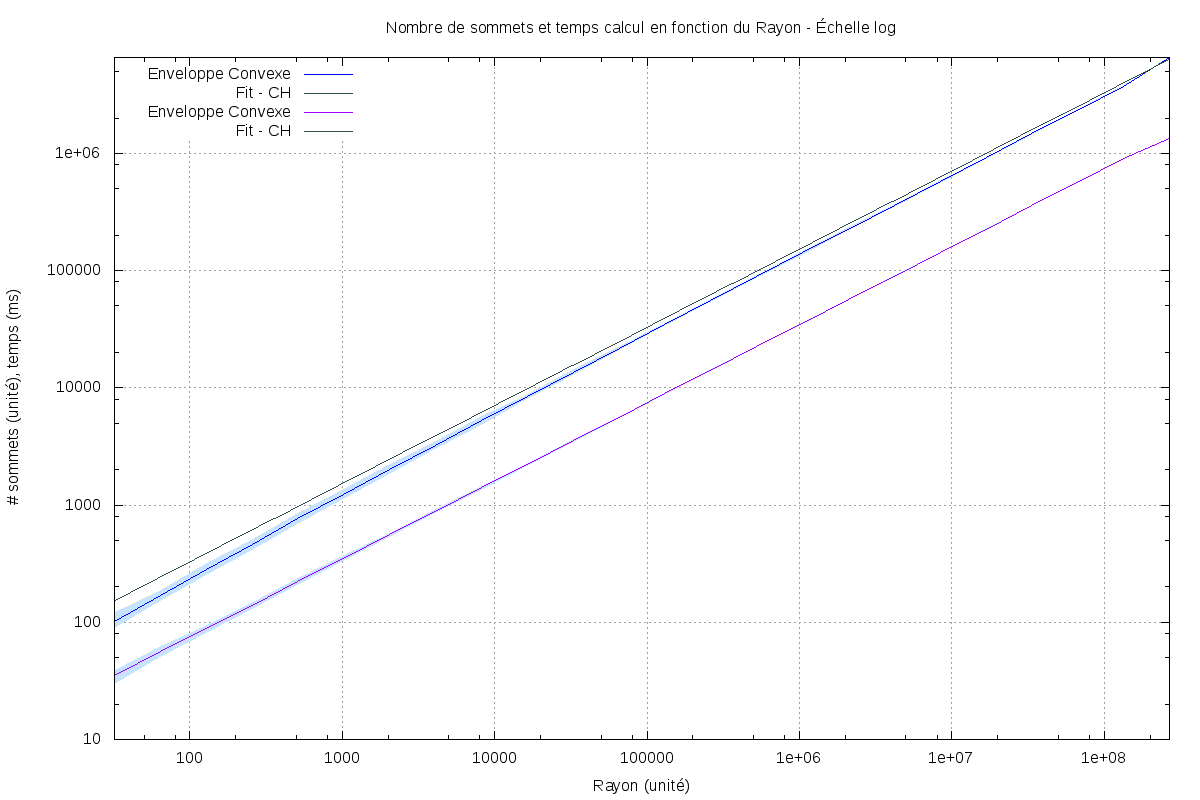
\includegraphics[width=\linewidth]{fig/4-exi/ch/exi-ch-sommet.png}
  \caption{Nombre de sommets de l'$\alpha$-shape en fonction de la taille des rayons. (Échelle log)}
\end{figure}


\begin{table}[H]
  \begin{tabular}{|p{0.09\linewidth}|p{0.13\linewidth}||p{0.23\linewidth}||p{0.23\linewidth}|p{0.23\linewidth}|}
    \hline
    \multicolumn{2}{|c||}{Rayon} & prédicat               & \multicolumn{2}{|c|}{$\alpha-shape$} \\  \hline 
    $R=2^k$  &                   & $-alpha = k*R^{2}$ & \multicolumn{2}{|c|}{Nombre de sommets} \\ \hline
    k        & R                 &                        & \# & $\# / R^{2/3}$ \\ 
    \hline
    
    \hline
  \end{tabular} 
  \caption{Nombre de sommets de l'$\alpha$-shape}
\end{table}
